% Options for packages loaded elsewhere
\PassOptionsToPackage{unicode}{hyperref}
\PassOptionsToPackage{hyphens}{url}
%
\documentclass[
  doc]{apa7}
\usepackage{amsmath,amssymb}
\usepackage{iftex}
\ifPDFTeX
  \usepackage[T1]{fontenc}
  \usepackage[utf8]{inputenc}
  \usepackage{textcomp} % provide euro and other symbols
\else % if luatex or xetex
  \usepackage{unicode-math} % this also loads fontspec
  \defaultfontfeatures{Scale=MatchLowercase}
  \defaultfontfeatures[\rmfamily]{Ligatures=TeX,Scale=1}
\fi
\usepackage{lmodern}
\ifPDFTeX\else
  % xetex/luatex font selection
\fi
% Use upquote if available, for straight quotes in verbatim environments
\IfFileExists{upquote.sty}{\usepackage{upquote}}{}
\IfFileExists{microtype.sty}{% use microtype if available
  \usepackage[]{microtype}
  \UseMicrotypeSet[protrusion]{basicmath} % disable protrusion for tt fonts
}{}
\makeatletter
\@ifundefined{KOMAClassName}{% if non-KOMA class
  \IfFileExists{parskip.sty}{%
    \usepackage{parskip}
  }{% else
    \setlength{\parindent}{0pt}
    \setlength{\parskip}{6pt plus 2pt minus 1pt}}
}{% if KOMA class
  \KOMAoptions{parskip=half}}
\makeatother
\usepackage{xcolor}
\usepackage{longtable,booktabs,array}
\usepackage{calc} % for calculating minipage widths
% Correct order of tables after \paragraph or \subparagraph
\usepackage{etoolbox}
\makeatletter
\patchcmd\longtable{\par}{\if@noskipsec\mbox{}\fi\par}{}{}
\makeatother
% Allow footnotes in longtable head/foot
\IfFileExists{footnotehyper.sty}{\usepackage{footnotehyper}}{\usepackage{footnote}}
\makesavenoteenv{longtable}
\usepackage{graphicx}
\makeatletter
\def\maxwidth{\ifdim\Gin@nat@width>\linewidth\linewidth\else\Gin@nat@width\fi}
\def\maxheight{\ifdim\Gin@nat@height>\textheight\textheight\else\Gin@nat@height\fi}
\makeatother
% Scale images if necessary, so that they will not overflow the page
% margins by default, and it is still possible to overwrite the defaults
% using explicit options in \includegraphics[width, height, ...]{}
\setkeys{Gin}{width=\maxwidth,height=\maxheight,keepaspectratio}
% Set default figure placement to htbp
\makeatletter
\def\fps@figure{htbp}
\makeatother
\usepackage{soul}
\setlength{\emergencystretch}{3em} % prevent overfull lines
\providecommand{\tightlist}{%
  \setlength{\itemsep}{0pt}\setlength{\parskip}{0pt}}
\setcounter{secnumdepth}{5}
% Make \paragraph and \subparagraph free-standing
\ifx\paragraph\undefined\else
  \let\oldparagraph\paragraph
  \renewcommand{\paragraph}[1]{\oldparagraph{#1}\mbox{}}
\fi
\ifx\subparagraph\undefined\else
  \let\oldsubparagraph\subparagraph
  \renewcommand{\subparagraph}[1]{\oldsubparagraph{#1}\mbox{}}
\fi
\ifLuaTeX
\usepackage[bidi=basic]{babel}
\else
\usepackage[bidi=default]{babel}
\fi
\babelprovide[main,import]{english}
% get rid of language-specific shorthands (see #6817):
\let\LanguageShortHands\languageshorthands
\def\languageshorthands#1{}
% Manuscript styling
\usepackage{upgreek}
\captionsetup{font=singlespacing,justification=justified}

% Table formatting
\usepackage{longtable}
\usepackage{lscape}
% \usepackage[counterclockwise]{rotating}   % Landscape page setup for large tables
\usepackage{multirow}		% Table styling
\usepackage{tabularx}		% Control Column width
\usepackage[flushleft]{threeparttable}	% Allows for three part tables with a specified notes section
\usepackage{threeparttablex}            % Lets threeparttable work with longtable

% Create new environments so endfloat can handle them
% \newenvironment{ltable}
%   {\begin{landscape}\centering\begin{threeparttable}}
%   {\end{threeparttable}\end{landscape}}
\newenvironment{lltable}{\begin{landscape}\centering\begin{ThreePartTable}}{\end{ThreePartTable}\end{landscape}}

% Enables adjusting longtable caption width to table width
% Solution found at http://golatex.de/longtable-mit-caption-so-breit-wie-die-tabelle-t15767.html
\makeatletter
\newcommand\LastLTentrywidth{1em}
\newlength\longtablewidth
\setlength{\longtablewidth}{1in}
\newcommand{\getlongtablewidth}{\begingroup \ifcsname LT@\roman{LT@tables}\endcsname \global\longtablewidth=0pt \renewcommand{\LT@entry}[2]{\global\advance\longtablewidth by ##2\relax\gdef\LastLTentrywidth{##2}}\@nameuse{LT@\roman{LT@tables}} \fi \endgroup}

% \setlength{\parindent}{0.5in}
% \setlength{\parskip}{0pt plus 0pt minus 0pt}

% Overwrite redefinition of paragraph and subparagraph by the default LaTeX template
% See https://github.com/crsh/papaja/issues/292
\makeatletter
\renewcommand{\paragraph}{\@startsection{paragraph}{4}{\parindent}%
  {0\baselineskip \@plus 0.2ex \@minus 0.2ex}%
  {-1em}%
  {\normalfont\normalsize\bfseries\itshape\typesectitle}}

\renewcommand{\subparagraph}[1]{\@startsection{subparagraph}{5}{1em}%
  {0\baselineskip \@plus 0.2ex \@minus 0.2ex}%
  {-\z@\relax}%
  {\normalfont\normalsize\itshape\hspace{\parindent}{#1}\textit{\addperi}}{\relax}}
\makeatother

\makeatletter
\usepackage{etoolbox}
\patchcmd{\maketitle}
  {\section{\normalfont\normalsize\abstractname}}
  {\section*{\normalfont\normalsize\abstractname}}
  {}{\typeout{Failed to patch abstract.}}
\patchcmd{\maketitle}
  {\section{\protect\normalfont{\@title}}}
  {\section*{\protect\normalfont{\@title}}}
  {}{\typeout{Failed to patch title.}}
\makeatother

\usepackage{xpatch}
\makeatletter
\xapptocmd\appendix
  {\xapptocmd\section
    {\addcontentsline{toc}{section}{\appendixname\ifoneappendix\else~\theappendix\fi\\: #1}}
    {}{\InnerPatchFailed}%
  }
{}{\PatchFailed}
\keywords{Schlüsselwort-XYZ}
\usepackage{csquotes}
\makeatletter
\renewcommand{\paragraph}{\@startsection{paragraph}{4}{\parindent}%
  {0\baselineskip \@plus 0.2ex \@minus 0.2ex}%
  {-1em}%
  {\normalfont\normalsize\bfseries\typesectitle}}

\renewcommand{\subparagraph}[1]{\@startsection{subparagraph}{5}{1em}%
  {0\baselineskip \@plus 0.2ex \@minus 0.2ex}%
  {-\z@\relax}%
  {\normalfont\normalsize\bfseries\itshape\hspace{\parindent}{#1}\textit{\addperi}}{\relax}}
\makeatother

\usepackage{times}
\babelprovide[main,import]{ngerman}
\usepackage{floatrow}
\floatsetup[figure]{capposition=top}
\floatsetup[table]{capposition=top}
\usepackage[backend=biber,style=apa]{biblatex}
\DeclareLanguageMapping{german}{german-apa}
\addbibresource{r-references.bib}
\DefineBibliographyStrings{ngerman}{references = {Literaturverzeichnis}}
\ifLuaTeX
  \usepackage{selnolig}  % disable illegal ligatures
\fi
\usepackage[]{biblatex}
\IfFileExists{bookmark.sty}{\usepackage{bookmark}}{\usepackage{hyperref}}
\IfFileExists{xurl.sty}{\usepackage{xurl}}{} % add URL line breaks if available
\urlstyle{same}
\hypersetup{
  pdftitle={APA Vorlage in deutscher Sprache},
  pdfauthor={Prof.~Dr.~Stephan Huber1,2 \& Vorname2 Nachname21},
  pdflang={en-EN},
  pdfkeywords={Schlüsselwort-XYZ},
  hidelinks,
  pdfcreator={LaTeX via pandoc}}

\title{APA Vorlage in deutscher Sprache}
\author{Prof.~Dr.~Stephan Huber\textsuperscript{1,2} \& Vorname2 Nachname2\textsuperscript{1}}
\date{}


\shorttitle{Kurztitel der Arbeit}

\authornote{

Alle Dateien im Zusammenhang mit diesem Dokument findet man hier: \url{https://github.com/hubchev/ewa/apa7vorlage}. Kontakt bitte über \texttt{stephan.huber@hs-fresenius.de} aufnehmen.

}

\affiliation{\vspace{0.5cm}\textsuperscript{1} Fresenius University of Applied Science\\\textsuperscript{2} Charlotte Fresenius University}

\abstract{%
Hier steht eine Zusammenfassung der Arbeit. Diese Manuskript macht inhaltlich keinen Sinn. Die entsprechend R Markdown Datei (.Rmd) soll lediglich das erstellen von APA (Version 7) konformen Manuskripten erleichtern. Ich versuche die wesentlichen Bestandteile von wissenschaftlichen Texten hier anzudeuten.
}



\begin{document}
\maketitle

\hypertarget{tabellen-und-grafiken}{%
\section{Tabellen und Grafiken}\label{tabellen-und-grafiken}}

Die Tabellen und Abbildungen sind als gleitende Einschübe im Haupttext erwähnt. So sind Abbildung \ref{fig:plotcar}, \ref{fig:pressure} und Tabelle \ref{tab:mixedtab} inhaltsfreie sind Beispiele die alle wesentliche Bestandteile enthalten. Will man noch eine Anmerkung unterhalb der Abbildung anbringen, wie von APA-7 empfohlen, muss etwas gebastelt werden. Das geht aber auch wie Abbildung \ref{fig:pressure} zeigt.

\begin{figure}
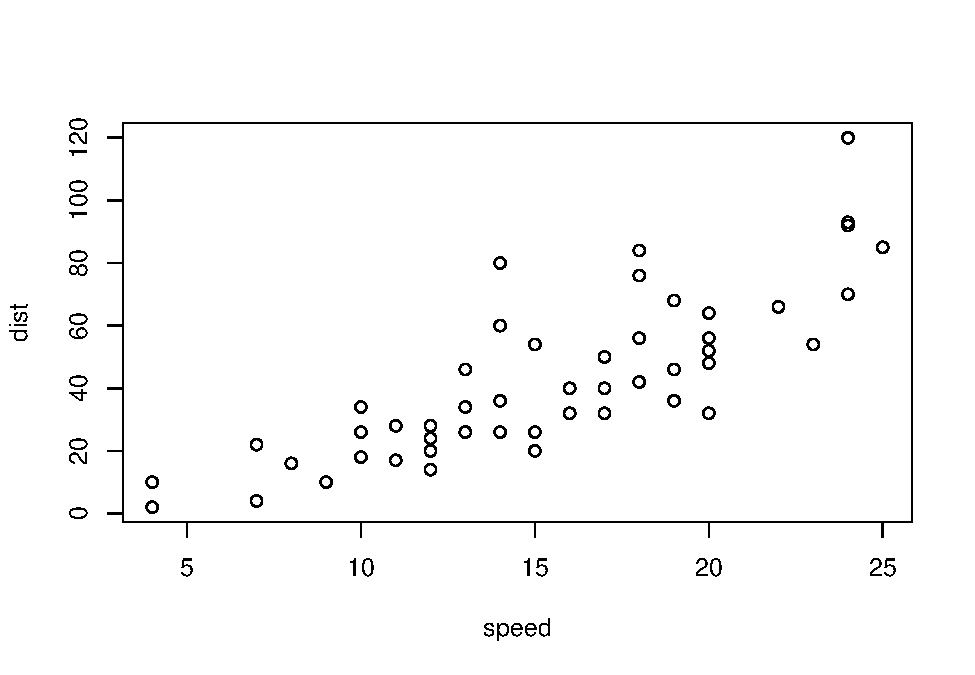
\includegraphics[width=.5\textwidth]{apa7vorlage_files/figure-latex/plotcar-1} \caption{Das ist ein gaaaaaaaaaaaaaaaaaaaaaaaaaaaaaaaaaaannnnnnnzzzz lange Überschrift für eine hässliche Abbildung.}\label{fig:plotcar}
\end{figure}

\begin{figure}[t]

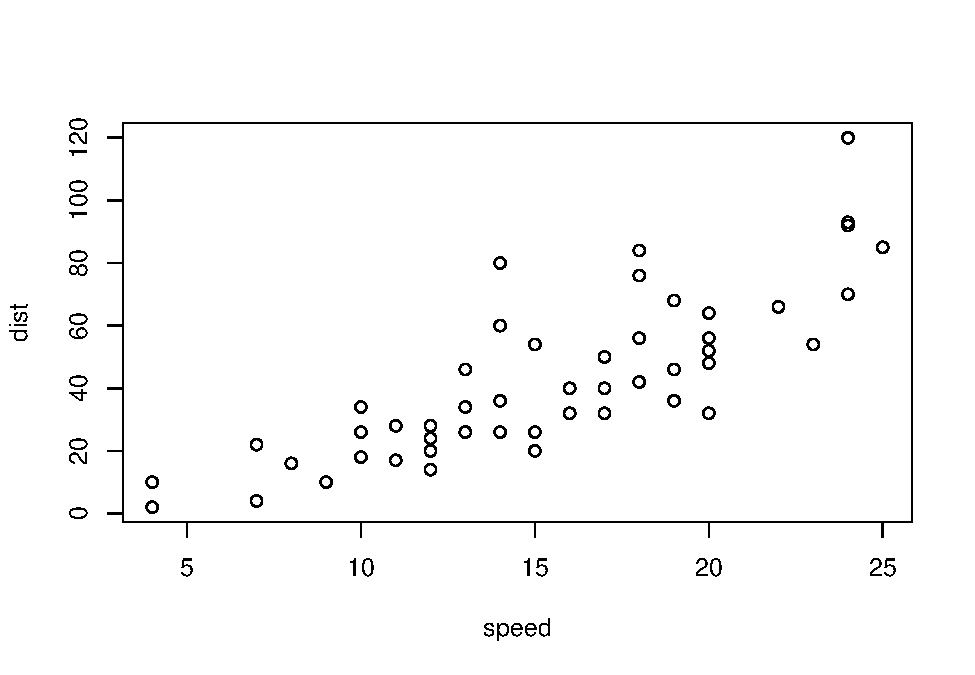
\includegraphics{apa7vorlage_files/figure-latex/pressure-1.pdf}

\caption{Das ist eine Grafik. \label{fig:pressure}}
\textit{Anmerkungen:} Hier kann man etwas anmerken.
\end{figure}

\begin{table}[tbp]

\begin{center}
\begin{threeparttable}

\caption{\label{tab:mixedtab}Ein Tabelle mit deskriptiver Statistik.}

\begin{tabular}{llllll}
\toprule
Dosage & \multicolumn{1}{c}{Mean} & \multicolumn{1}{c}{Median} & \multicolumn{1}{c}{SD} & \multicolumn{1}{c}{Min} & \multicolumn{1}{c}{Max}\\
\midrule
A & 14.19 & 14.00 & 4.45 & 5 & 25\\
B & 13.50 & 14.00 & 5.15 & 4 & 22\\
C & 19.19 & 19.00 & 3.52 & 13 & 25\\
\bottomrule
\addlinespace
\end{tabular}

\begin{tablenotes}[para]
\normalsize{\textit{Anmerkungen.} Diese Tabelle wurde mit apa\_table() erstellt.}
\end{tablenotes}

\end{threeparttable}
\end{center}

\end{table}

\hypertarget{zitieren}{%
\section{Zitieren}\label{zitieren}}

In wissenschaftlichen Texten werden oft andere Arbeiten zitiert. Dies kann auf unterschiedlichste Weise geschehen. Tabelle \ref{tbl-letters} zeigt, wie zitiert werden kann.

\begin{longtable}[]{@{}
  >{\raggedright\arraybackslash}p{(\columnwidth - 2\tabcolsep) * \real{0.5294}}
  >{\raggedright\arraybackslash}p{(\columnwidth - 2\tabcolsep) * \real{0.4706}}@{}}
\caption{So kann Literatur zitiert werden \label{tbl-letters}}\tabularnewline
\toprule\noalign{}
\begin{minipage}[b]{\linewidth}\raggedright
Code
\end{minipage} & \begin{minipage}[b]{\linewidth}\raggedright
So erscheint es im Text
\end{minipage} \\
\midrule\noalign{}
\endfirsthead
\toprule\noalign{}
\begin{minipage}[b]{\linewidth}\raggedright
Code
\end{minipage} & \begin{minipage}[b]{\linewidth}\raggedright
So erscheint es im Text
\end{minipage} \\
\midrule\noalign{}
\endhead
\bottomrule\noalign{}
\endlastfoot
\texttt{@Zank2022Quality} & \textcite{Zank2022Quality} \\
\texttt{@Zank2022Quality{[}S.\ 6{]}} & \textcite[S. 6]{Zank2022Quality} \\
\texttt{{[}@Zank2022Quality{]}} & \autocite{Zank2022Quality} \\
\texttt{{[}@Zank2022Quality,\ S.\ 7{]}} & \autocite[S. 7]{Zank2022Quality} \\
\texttt{{[}@Zank2022Quality;\ @Aust2020papaja{]}} & \autocite{Zank2022Quality,Aust2020papaja} \\
\texttt{{[}Vgl.\ @Zank2022Quality,\ S.\ 31;\ @Aust2020papaja,\ S.\ 13{]}} & \autocites[Vgl.][S. 31]{Zank2022Quality}[S. 13]{Aust2020papaja} \\
\end{longtable}

Hyperlinks kann man auch setzen: \texttt{{[}Google{]}(www.google.de)} wird zu: \href{www.google.de}{Google}.
Bei akademischen Arbeiten sollten Quellen immer in das Literaturverzeichnis und Hyperlinks funktionieren nicht in gedruckter Form. Hier ein Beispiel: \href{www.google.de}{Google} ist eine beliebte Online-Suchmaschine \autocite[siehe][]{Google2023Google}.

\hypertarget{kapitel}{%
\section{Kapitel}\label{kapitel}}

Die Formatierung der Überschriften regelt APA strikt, siehe:
\url{https://apastyle.apa.org/style-grammar-guidelines/paper-format/headings}

\hypertarget{abschnitt}{%
\subsection{Abschnitt}\label{abschnitt}}

\hypertarget{das-ist-unterabschnitt}{%
\subsubsection{Das ist Unterabschnitt}\label{das-ist-unterabschnitt}}

Ein Abschnitt sollte nicht alleine kommen, daher\ldots{}

\hypertarget{der-zweite-unterabschnitt}{%
\subsubsection{Der zweite Unterabschnitt}\label{der-zweite-unterabschnitt}}

Hier gehört ihr Text.

\hypertarget{die-vierte-gliederungsebene}{%
\paragraph{Die vierte Gliederungsebene}\label{die-vierte-gliederungsebene}}

Sollte nicht durch einen Zeilenumbruch vom Text getrennt sein.

\hypertarget{text-formatieren}{%
\section{Text formatieren}\label{text-formatieren}}

\textbf{This is bold text}

\textbf{This is bold text}

\emph{This is italic text}

\emph{This is italic text}

\st{Strikethrough}

\hypertarget{listen}{%
\subsection{Listen}\label{listen}}

\begin{itemize}
\tightlist
\item
  Eine Liste erstellen, indem man eine Zeile mit \texttt{+}, \texttt{-} oder \texttt{*} beginnt
\item
  Unterlisten werden durch Einrücken um 2 Leerzeichen erstellt:

  \begin{itemize}
  \tightlist
  \item
    Ein Wechsel des Markierungszeichens erzwingt den Start einer neuen Liste:

    \begin{itemize}
    \tightlist
    \item
      bli
    \item
      bla
    \item
      blubb
    \end{itemize}
  \end{itemize}
\item
  Sehr einfach!
\end{itemize}

Nummerierte Listen sind einfach:

\begin{enumerate}
\def\labelenumi{\arabic{enumi}.}
\item
  Ein Argument.
\item
  Ein weiteres Argument.
\item
  Das beste Argument.
\item
  Man kann fortlaufende Zahlen verwenden\ldots{}
\item
  \ldots oder alle Zahlen als \texttt{1.} behalten
\end{enumerate}

Nummerierung mit einer höheren Zahl beginnen, geht auch:

\begin{enumerate}
\def\labelenumi{\arabic{enumi}.}
\setcounter{enumi}{56}
\tightlist
\item
  foo
\item
  bar
\end{enumerate}

\hypertarget{code}{%
\subsection{Code}\label{code}}

Inline \texttt{code}

Eingerückter Code

\begin{verbatim}
// Einige Kommentare
Zeile 1 des Codes
Zeile 2 des Codes
Zeile 3 des Codes
\end{verbatim}

\hypertarget{bilder-einfuxfcgen}{%
\subsection{Bilder einfügen}\label{bilder-einfuxfcgen}}

In Abbildung \ref{fig:figofme} zeige ich wie eine .jpeg Datei in eine Abbildung eingefügt werden kann.

\begin{figure}

{\centering 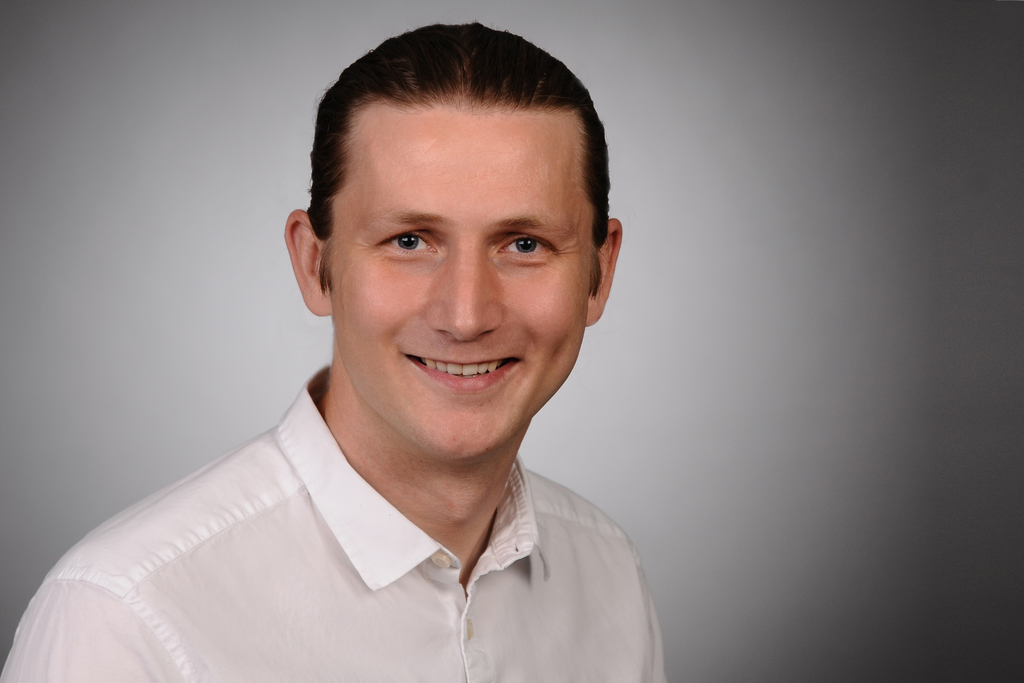
\includegraphics[width=0.2\linewidth]{temp} 

}

\caption{This is a smaller picture of me}\label{fig:figofme}
\end{figure}

\hypertarget{formeln}{%
\subsection{Formeln}\label{formeln}}

Wenn \(a \ne 0\) ist, gibt es zwei Lösungen für die Gleichung \((ax^2 + bx + c = 0)\) und sie lauten
\[ x = \frac{-b \pm \sqrt{b^2-4ac}}{2a} \]

\hypertarget{fuuxdfnoten}{%
\subsection{\texorpdfstring{\href{https://github.com/markdown-it/markdown-it-footnote}{Fußnoten}}{Fußnoten}}\label{fuuxdfnoten}}

Fußnote 1 Verweis\footnote{Fußnote \textbf{kann Markup enthalten}

  und mehrere Absätze.}.

Fußnote 2 Verweis\footnote{Fußnotentext.}.

Inline Fußnote\footnote{Text der Inline-Fußnote} Definition.

Doppelter Fußnotenverweis\footnote{Fußnotentext.}.

\printbibliography

\newpage

\hypertarget{appendix-appendix}{%
\appendix}


\hypertarget{das-ist-der-erste-anhang}{%
\section{Das ist der erste Anhang}\label{das-ist-der-erste-anhang}}

Hier befindet sich Abbildung \ref{fig:plotcar2}.

\begin{figure}
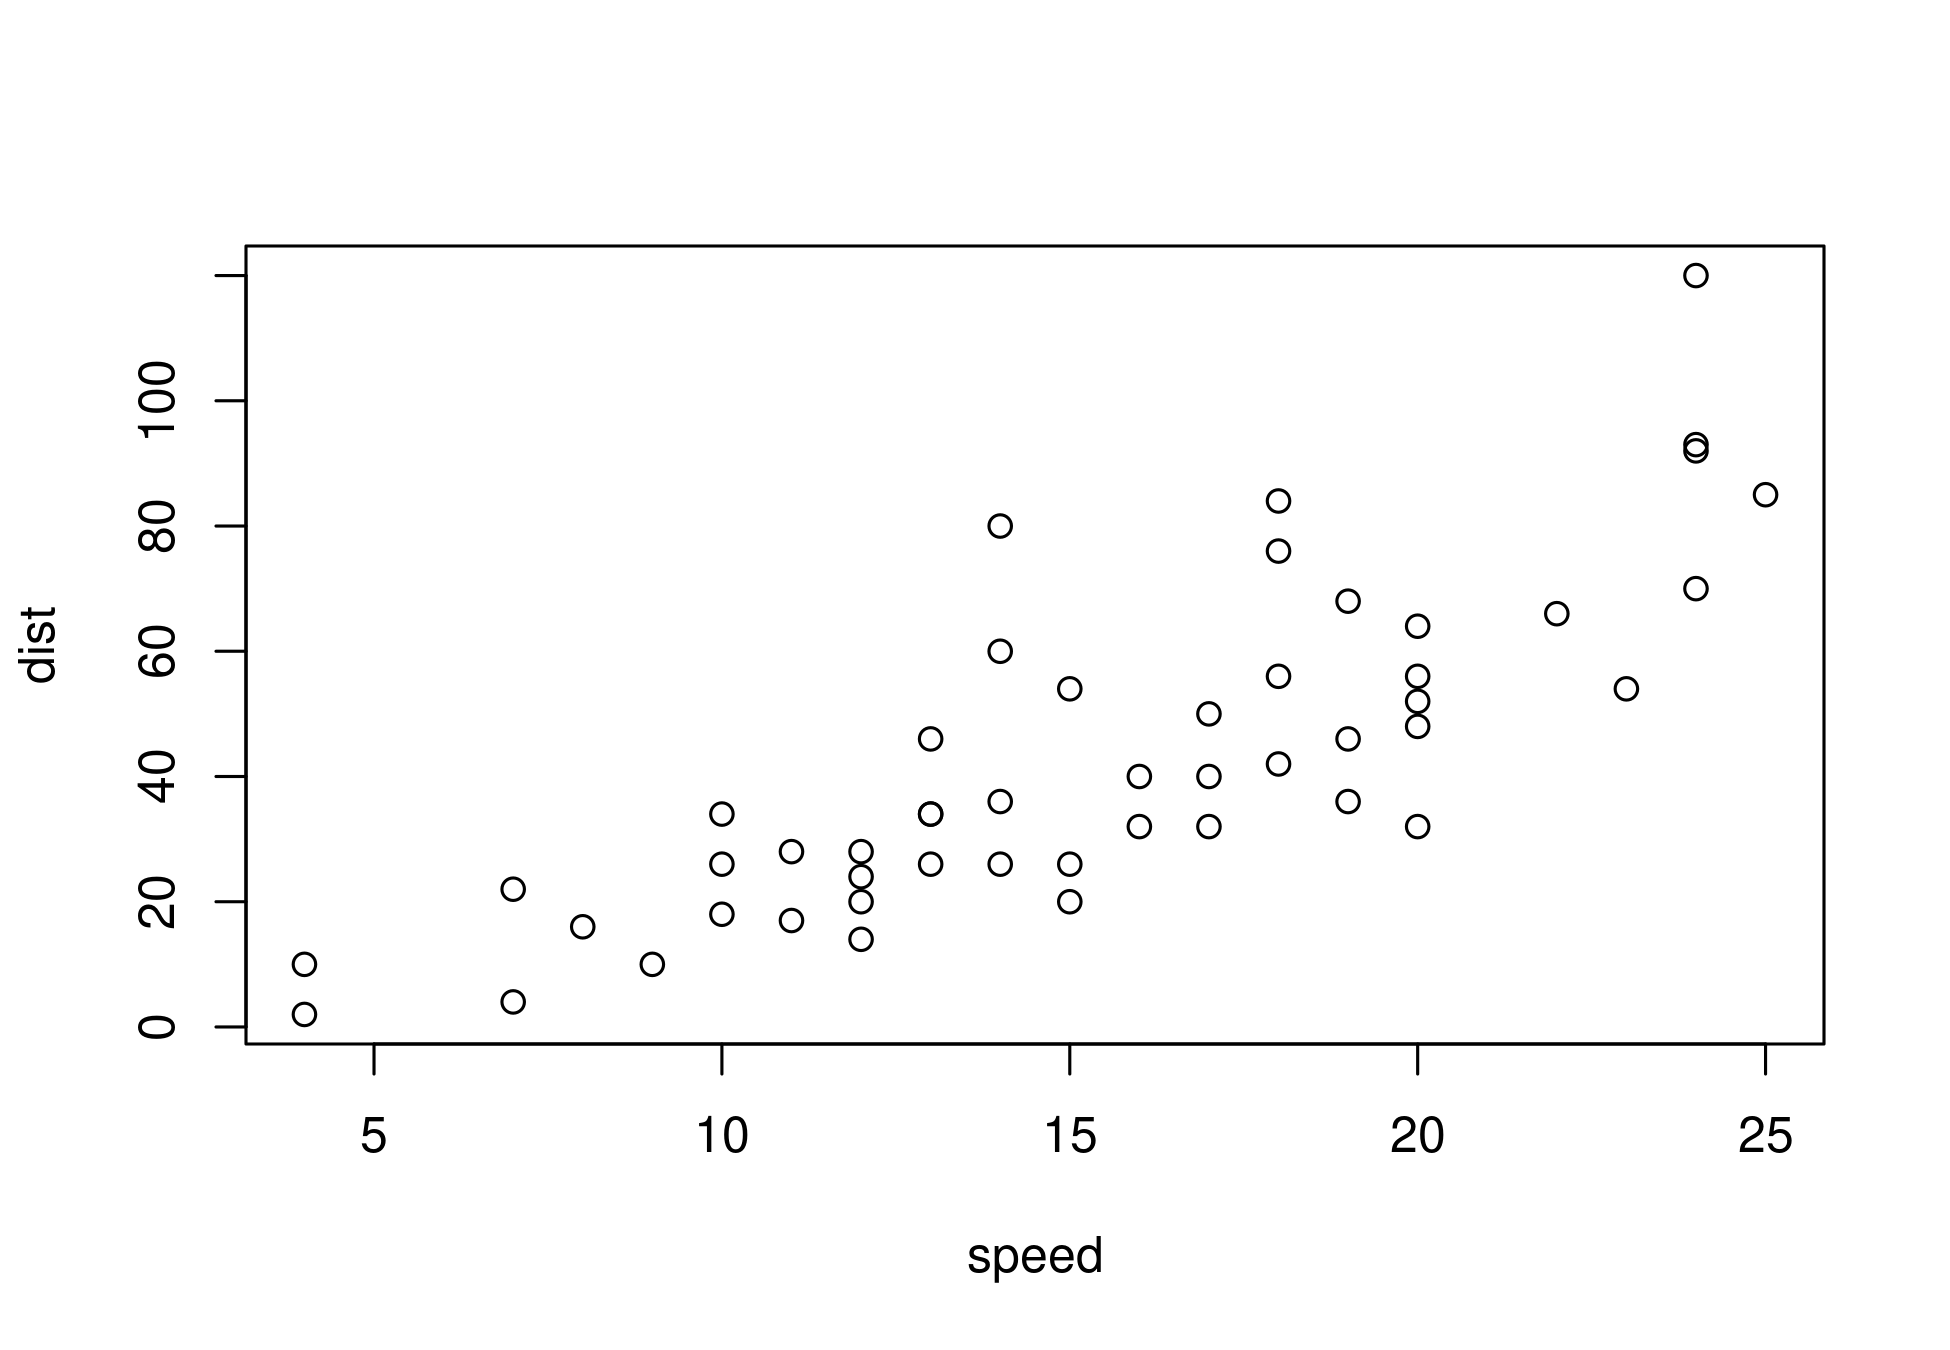
\includegraphics[width=0.1\textwidth]{apa7vorlage_files/figure-latex/plotcar2-1} \caption{Das ist ein gaaaaaaaaaaaaaaaaaaaaaaaaaaaaaaaaaaannnnnnnzzzz lange Überschrift für eine Abbildung.}\label{fig:plotcar2}
\end{figure}

\hypertarget{das-literaturverzeichnis-nochmal-anzeigen-oder-nicht}{%
\section{Das Literaturverzeichnis nochmal anzeigen oder nicht?}\label{das-literaturverzeichnis-nochmal-anzeigen-oder-nicht}}

Standardmäßig wird das Literaturverzeichnis im Anhang wiederholt. Wer das nicht will kann das mit

\texttt{\textbackslash{}renewcommand\{\textbackslash{}printbibliography\}\{\}}

unterdrücken.

\renewcommand{\printbibliography}{}


\printbibliography

\end{document}
